The first attempt of generation of artificial scans was based on Variational Autoencoder architecture proposed in the \cite{rombach2022high}. Implementation was based on Monai\cite{Cardoso_MONAI_An_open-source_2022} example available on Github\footnote{\url{https://github.com/Project-MONAI/GenerativeModels/blob/e7cc989cdce440a7bff1cce22fff1caf760f39cd/tutorials/generative/3d_autoencoderkl/3d_autoencoderkl_tutorial.ipynb}} and adjusted to Pytorch Lightning. The final implementation is available in the project repository in file.

\paragraph{Model configuration}

\paragraph{Training}

\begin{figure}[H]
\minipage{0.49\textwidth}
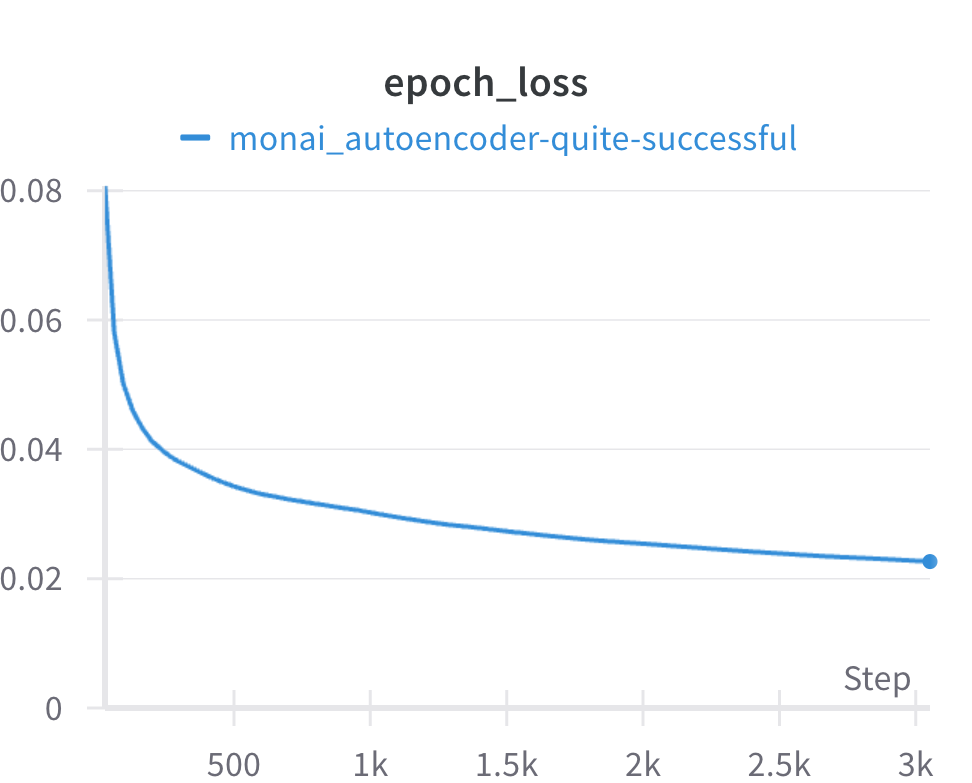
\includegraphics[width=\linewidth]{detailed_engineering/Monai Autoencoder/charts/epoch_loss.png}
\caption{}
\endminipage\hfill
\minipage{0.49\textwidth}
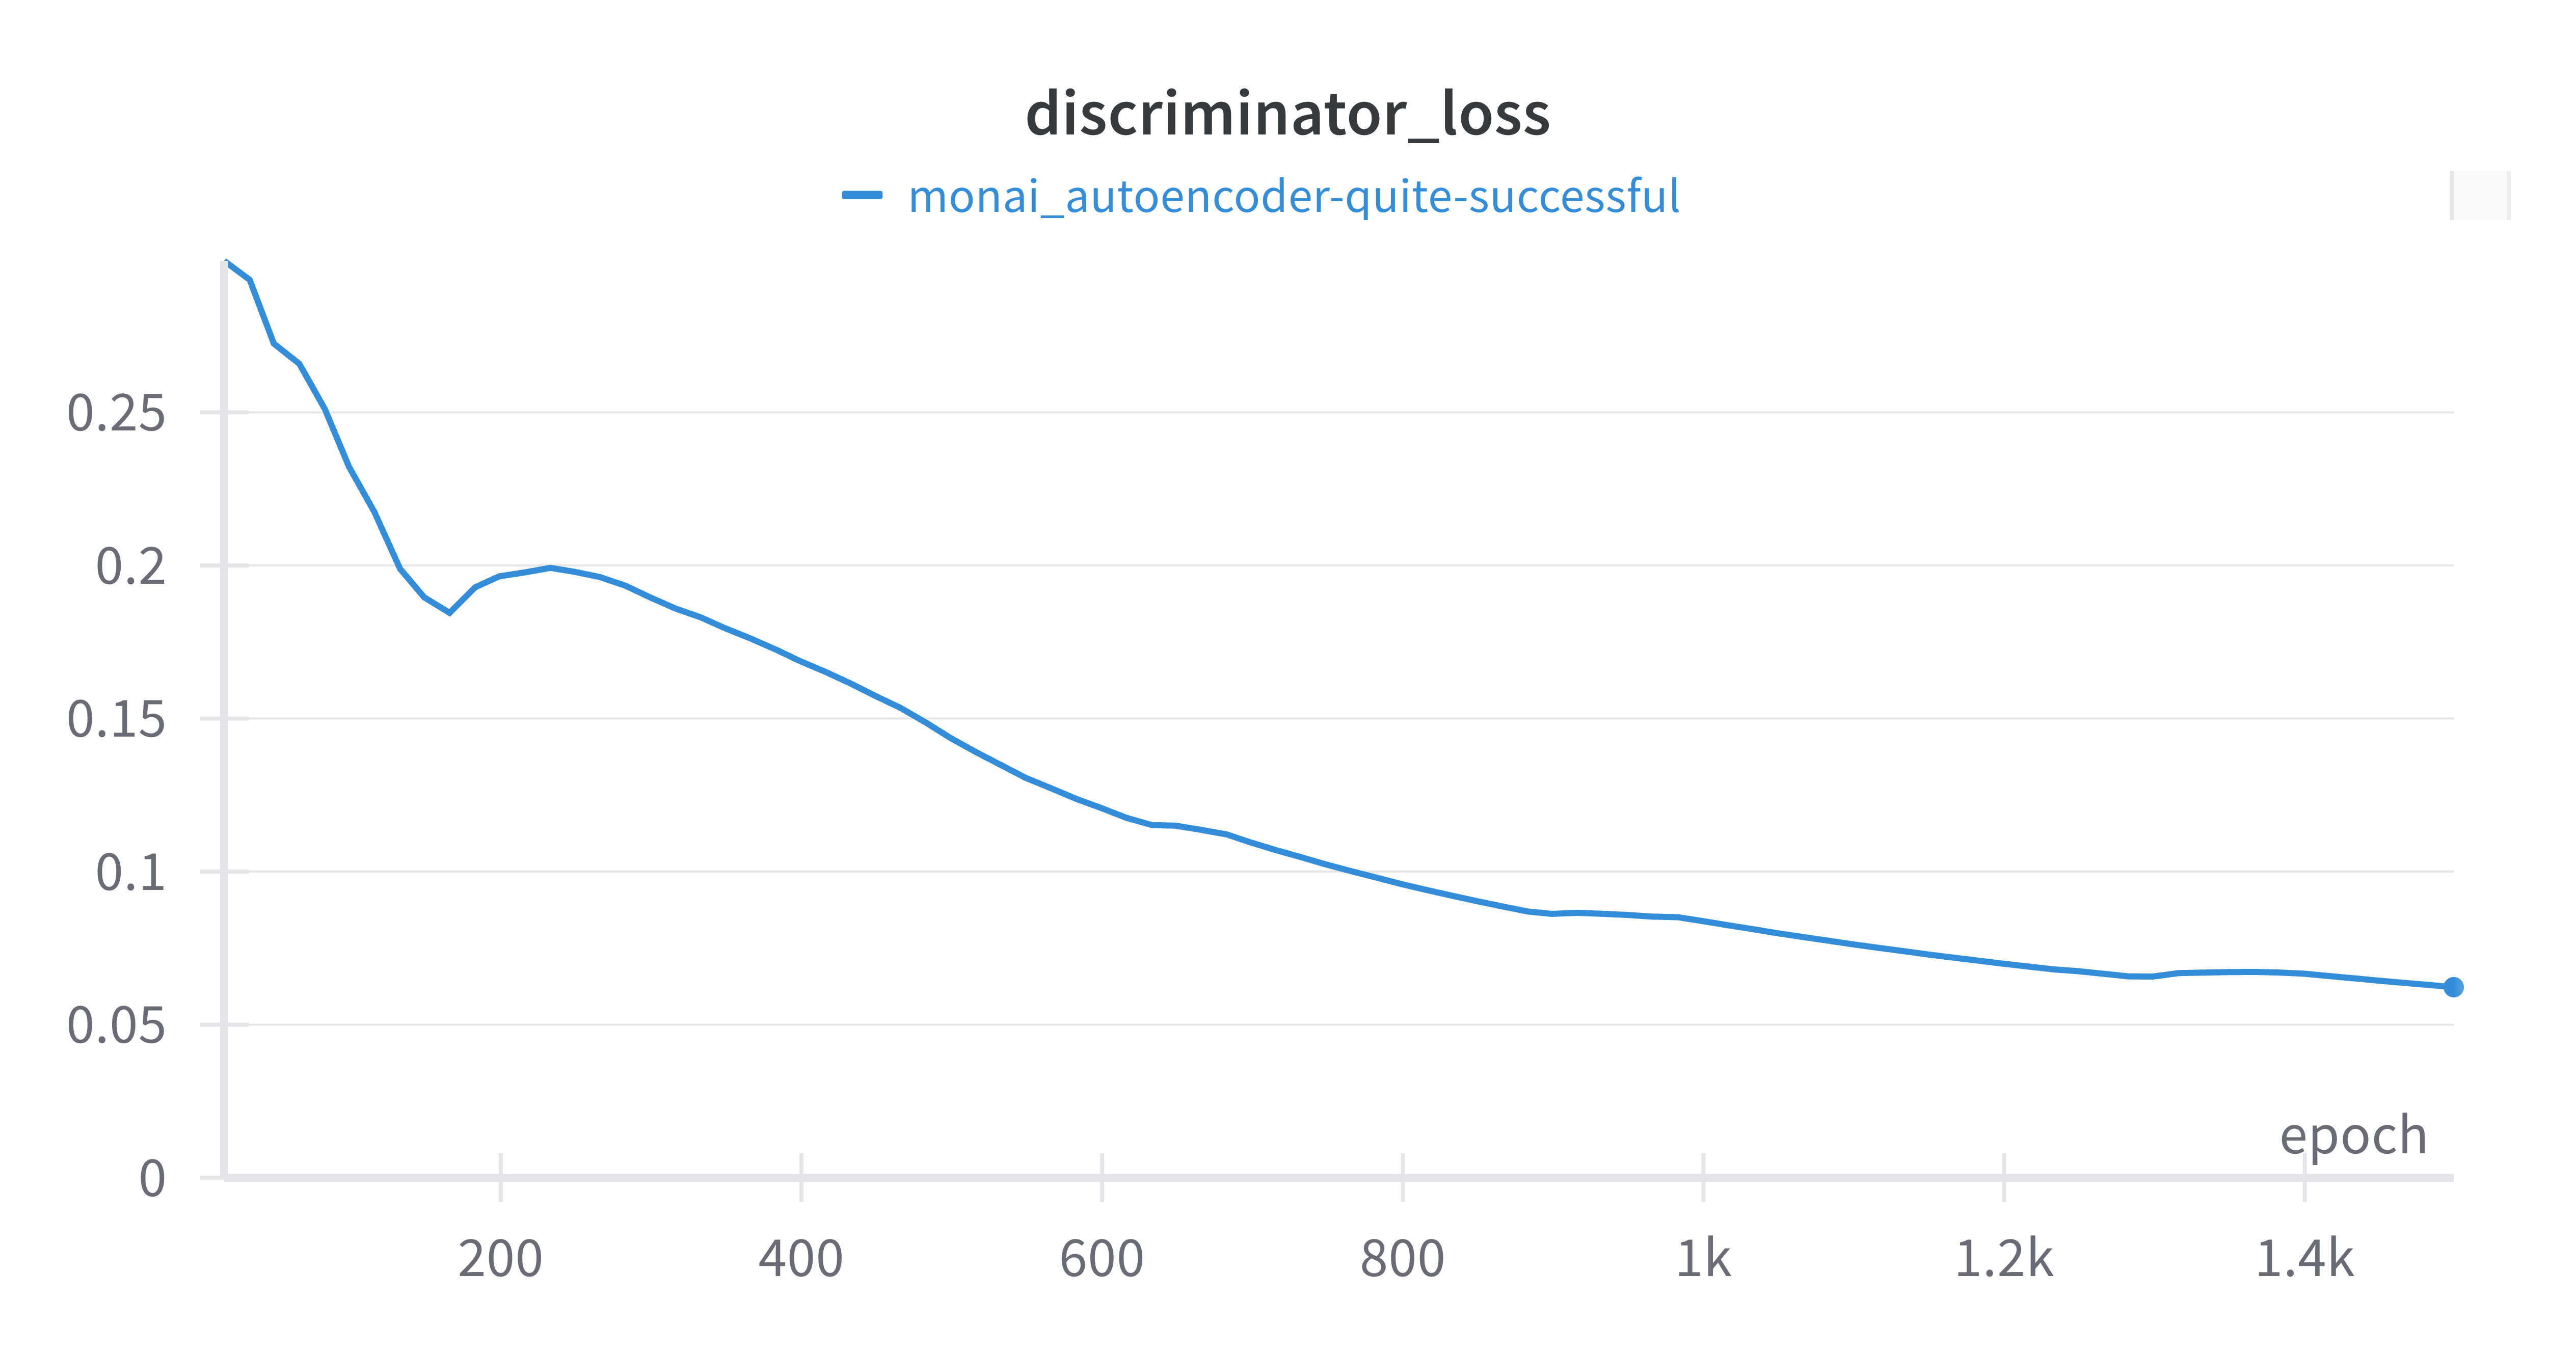
\includegraphics[width=\linewidth]{detailed_engineering/Monai Autoencoder/charts/discriminator_loss.png}
\caption{}
\endminipage
\end{figure}

\begin{figure}[H]
\minipage{0.49\textwidth}
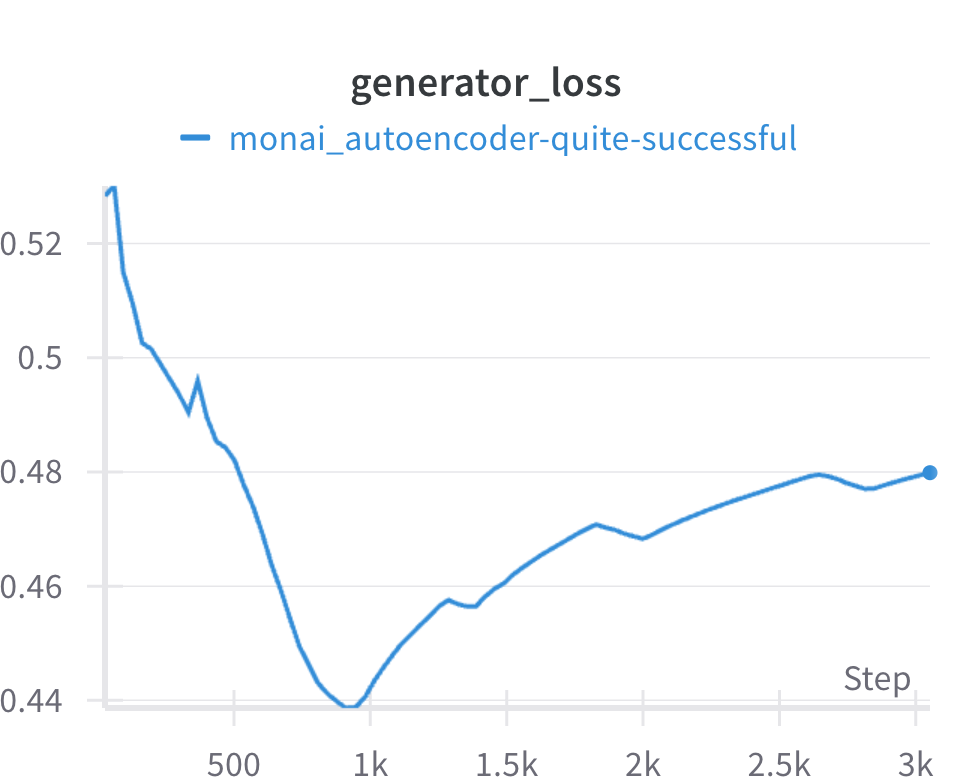
\includegraphics[width=\linewidth]{detailed_engineering/Monai Autoencoder/charts/generator_loss.png}
\caption{}
\endminipage\hfill
\minipage{0.49\textwidth}
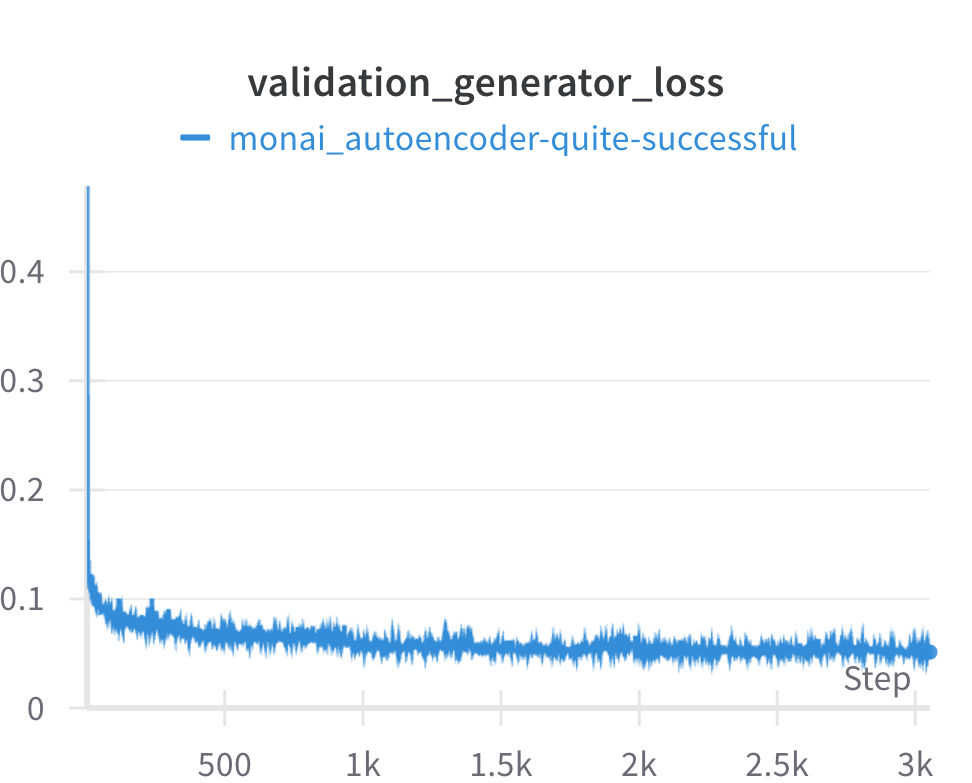
\includegraphics[width=\linewidth]{detailed_engineering/Monai Autoencoder/charts/val_generator_loss.png}
\caption{}
\endminipage
\end{figure}


\begin{figure}[H]
% \minipage{0.49\textwidth}
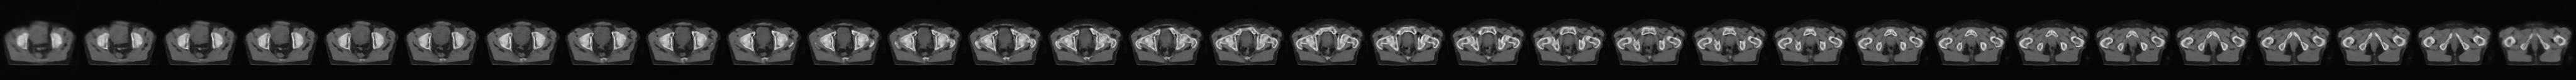
\includegraphics[width=\linewidth]{detailed_engineering/Monai Autoencoder/charts/reconstruction.png}
\caption{}
% \endminipage\hfill
% \minipage{0.49\textwidth}
% \includegraphics[width=\linewidth]{charts/Section-4-Panel-5-z2xepgyu7}
% \caption{}
% \endminipage
\end{figure}
d



% \begin{figure}[H]
% \centering
% \begin{subfigure}[h]{.45\linewidth}
%     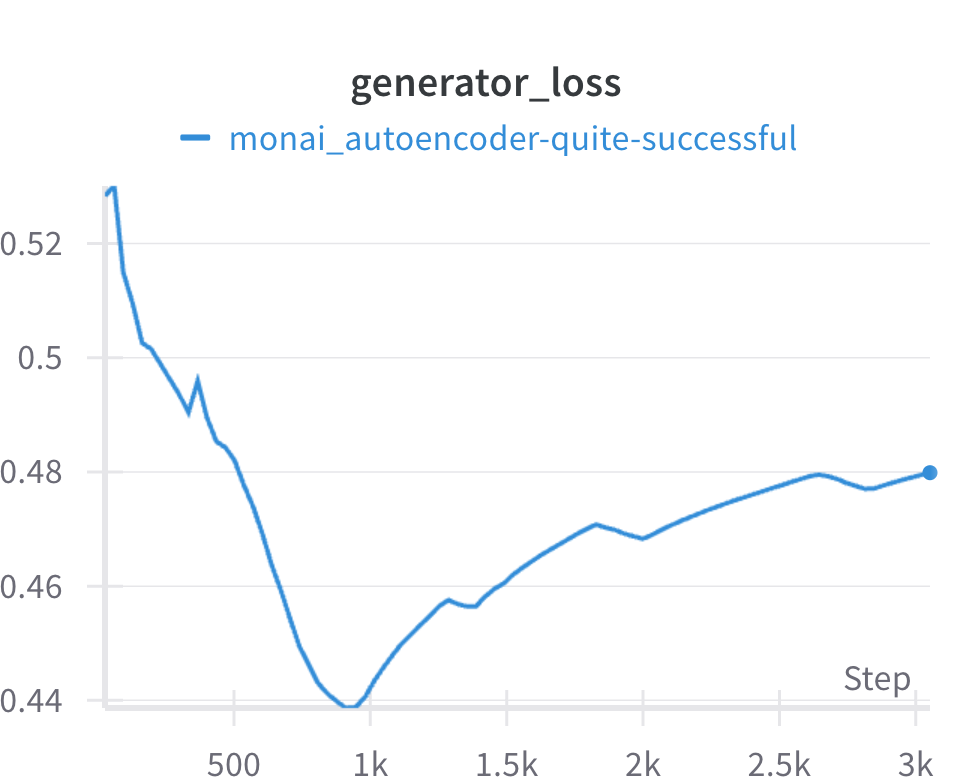
\includegraphics[width=\linewidth]{detailed_engineering/Monai Autoencoder/charts/generator_loss.png}
%     \caption{Caption}
%     \label{fig:enter-label}
% \end{subfigure}
% \hfill
% \begin{subfigure}[h]{.45\linewidth}
%     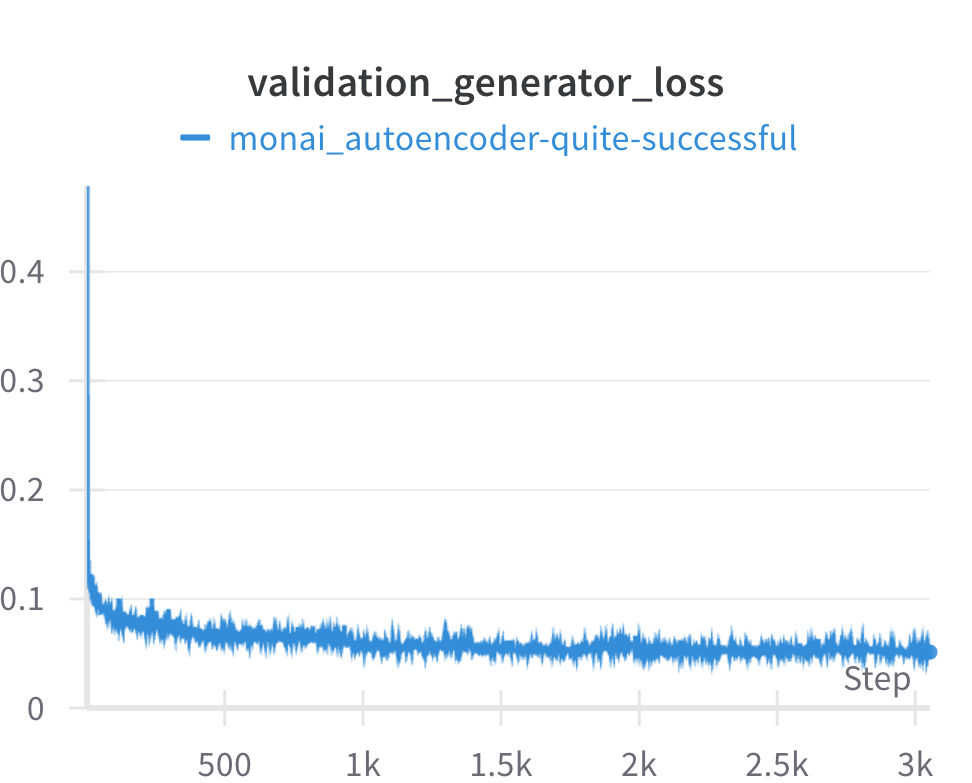
\includegraphics[width=\linewidth]{detailed_engineering/Monai Autoencoder/charts/val_generator_loss.png}
%     \caption{Caption}
%     \label{fig:enter-label}
% \end{subfigure}
% \hfill
% \begin{subfigure}[h]{.45\linewidth}
%     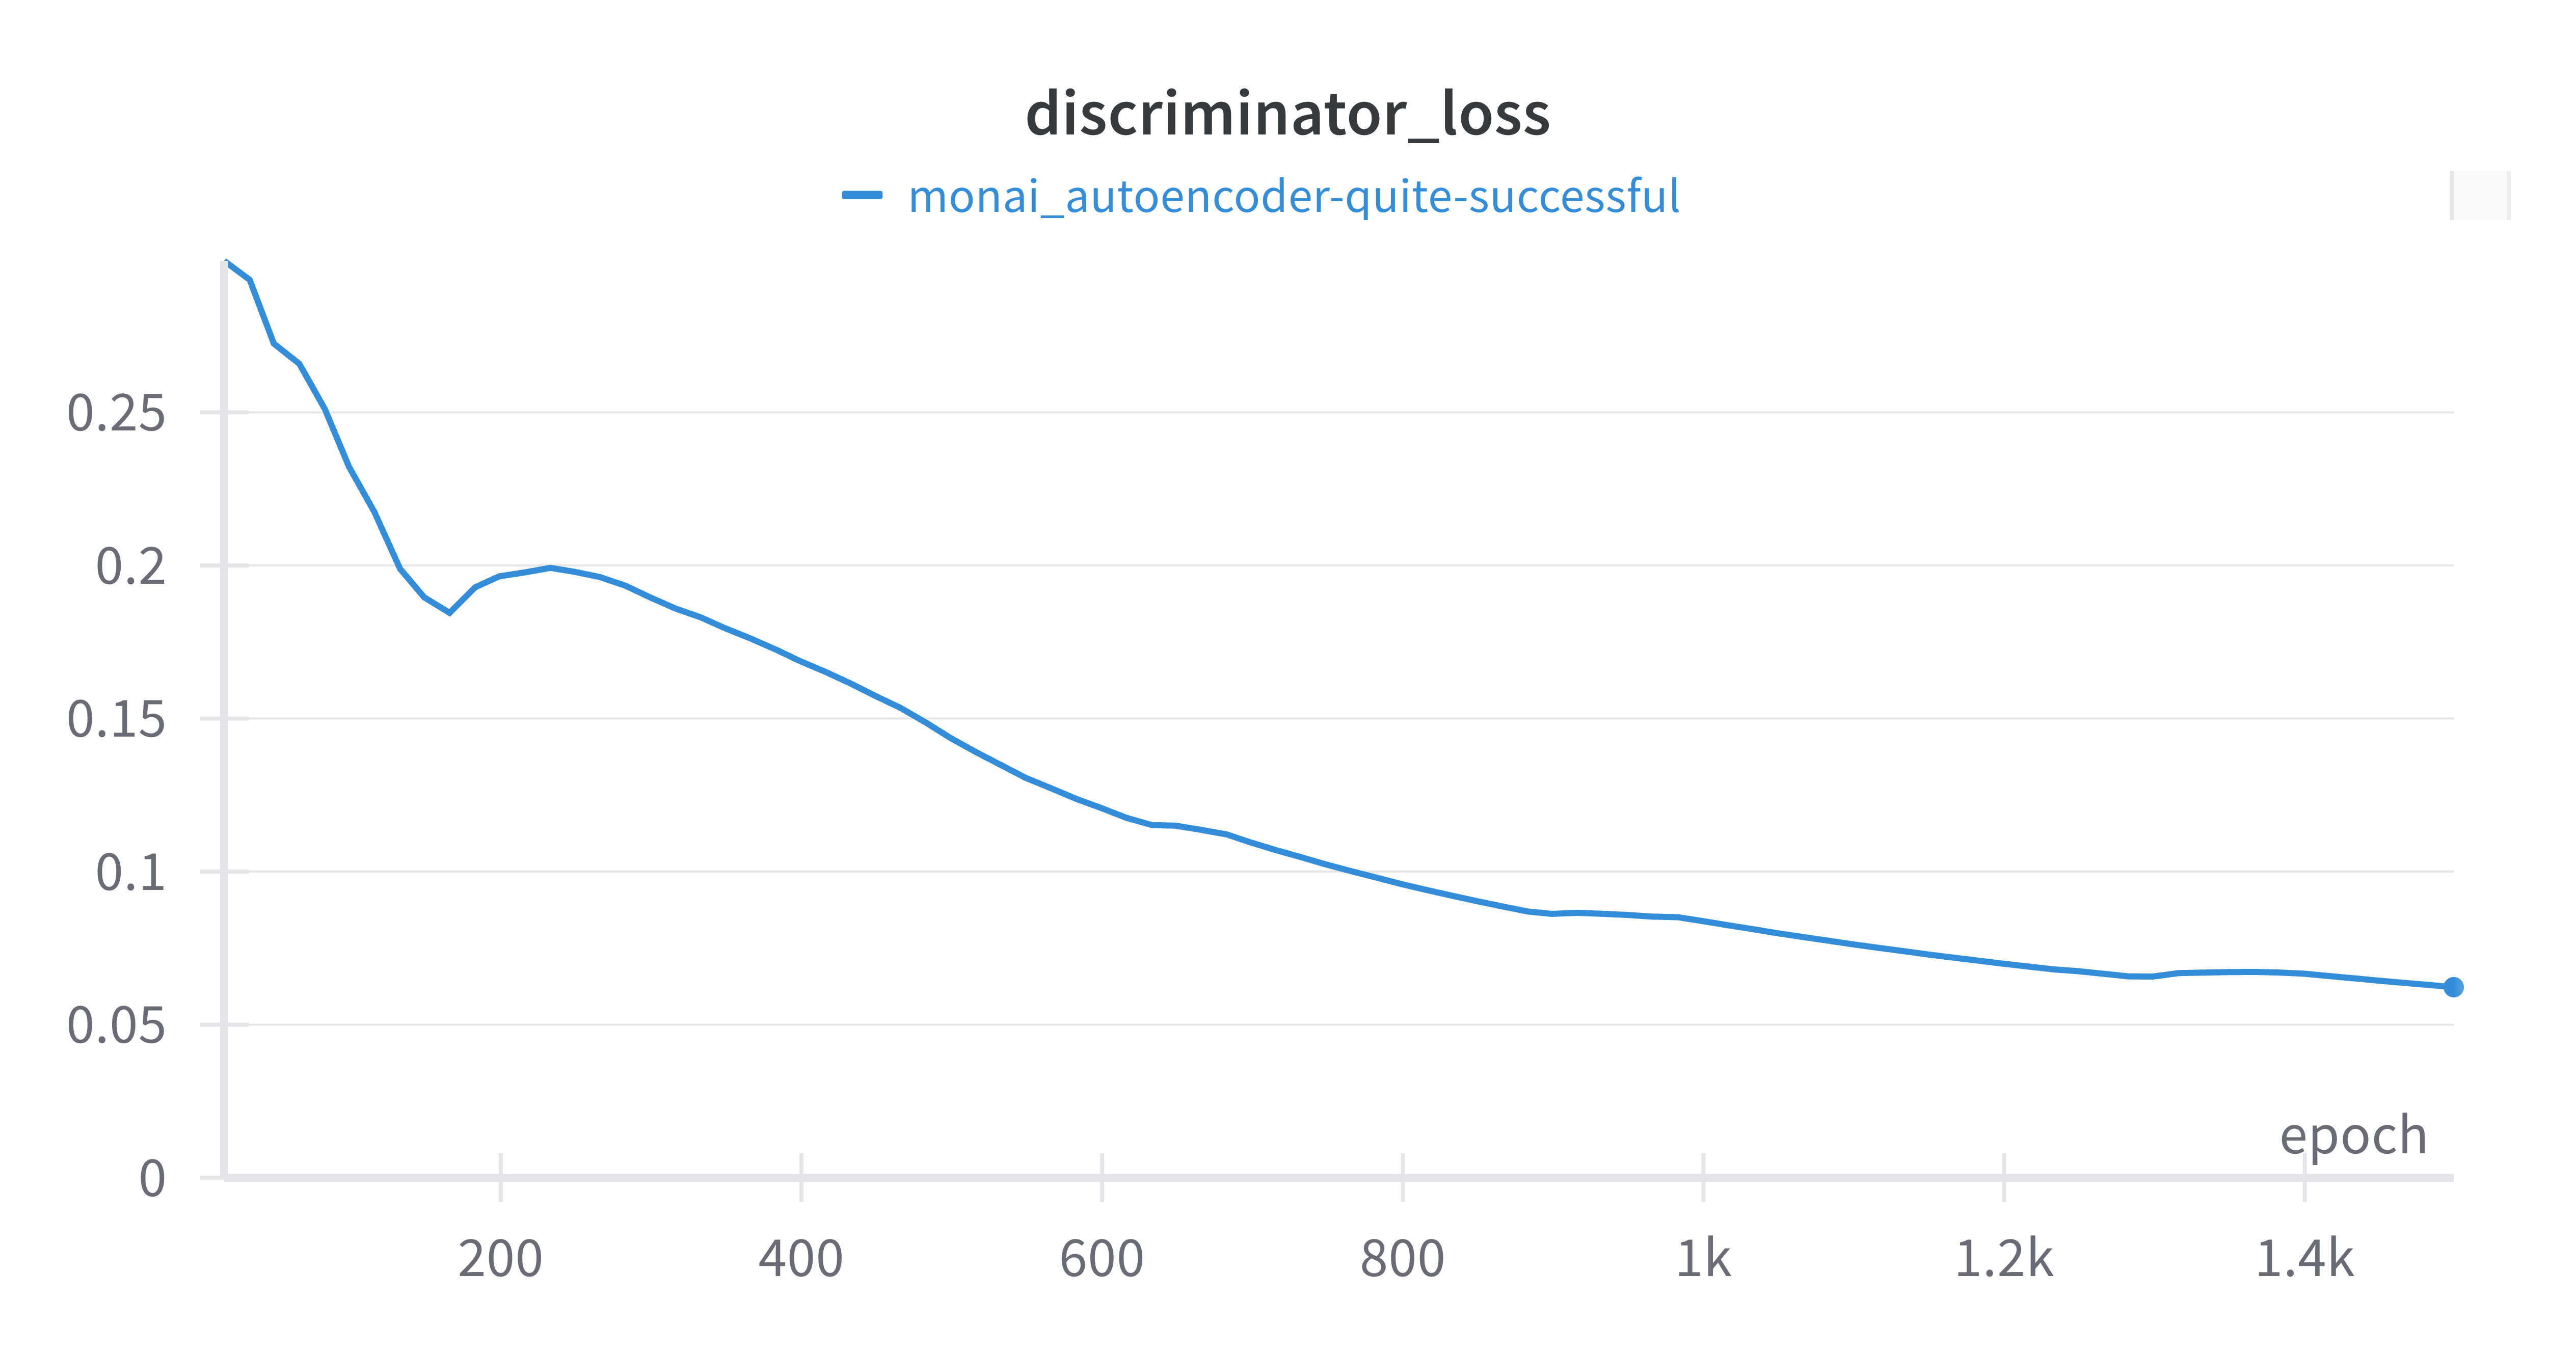
\includegraphics[width=\linewidth]{detailed_engineering/Monai Autoencoder/charts/discriminator_loss.png}
%     \caption{Caption}
%     \label{fig:enter-label}
% \end{subfigure}
% \hfill
% \begin{subfigure}[h]{.45\linewidth}
%     \includegraphics[width=\linewidth]{detailed_engineering/Monai Autoencoder/charts/Section-4-Panel-4-d216pe2qa.png}
%     \caption{Caption}
%     \label{fig:enter-label}
% \end{subfigure}
% \hfill
% \begin{subfigure}[h]{.45\linewidth}
%     \includegraphics[width=\linewidth]{detailed_engineering/Monai Autoencoder/charts/Section-4-Panel-5-z2xepgyu7.png}
%     \caption{Caption}
%     \label{fig:enter-label}
% \end{subfigure}
%\begin{subfigure}[b]
%     \includegraphics[width=0.5\linewidth]{detailed_engineering/Monai Autoencoder/charts/Section-4-Panel-2-bm1y05a9m.png}
%     \caption{Caption}
%     \label{fig:enter-label}
% \end{subfigure}
% \begin{subfigure}[b]
%     \includegraphics[width=0.5\linewidth]{detailed_engineering/Monai Autoencoder/charts/Section-4-Panel-3-dkwhik6ki.png}
%     \caption{Caption}
%     \label{fig:enter-label}
% \end{subfigure}
% \begin{subfigure}[b]
%     \includegraphics[width=0.5\linewidth]{detailed_engineering/Monai Autoencoder/charts/Section-4-Panel-4-d216pe2qa.png}
%     \caption{Caption}
%     \label{fig:enter-label}
% \end{subfigure}
% \begin{subfigure}[b]
%     \includegraphics[width=0.5\linewidth]{detailed_engineering/Monai Autoencoder/charts/Section-4-Panel-5-z2xepgyu7.png}
%     \caption{Caption}
%     \label{fig:enter-label}
% \end{subfigure}
% \end{figure}


\paragraph{Results}


\paragraph{LDM model for VAE}

\paragraph{LDM Attempt 2}\mbox{}\\

\indent In this attempt instead of creating noise from $\sim\mathcal{N}(0,1)$, the noise was generated from $N(\mu, \sigma)$ where $\mu$ is the mean of the training data $z_{\mu}$ and $\sigma$ is the mean of $z_{\sigma}$ obtained from the training data set (25 samples).

\paragraph{Model configuration}\mbox{}\\
The configuration was the same as in Attempt 1. The only difference was in the noise generation approach.

\paragraph{Training}\mbox{}\\
\begin{figure}[H]
\minipage{0.49\textwidth}
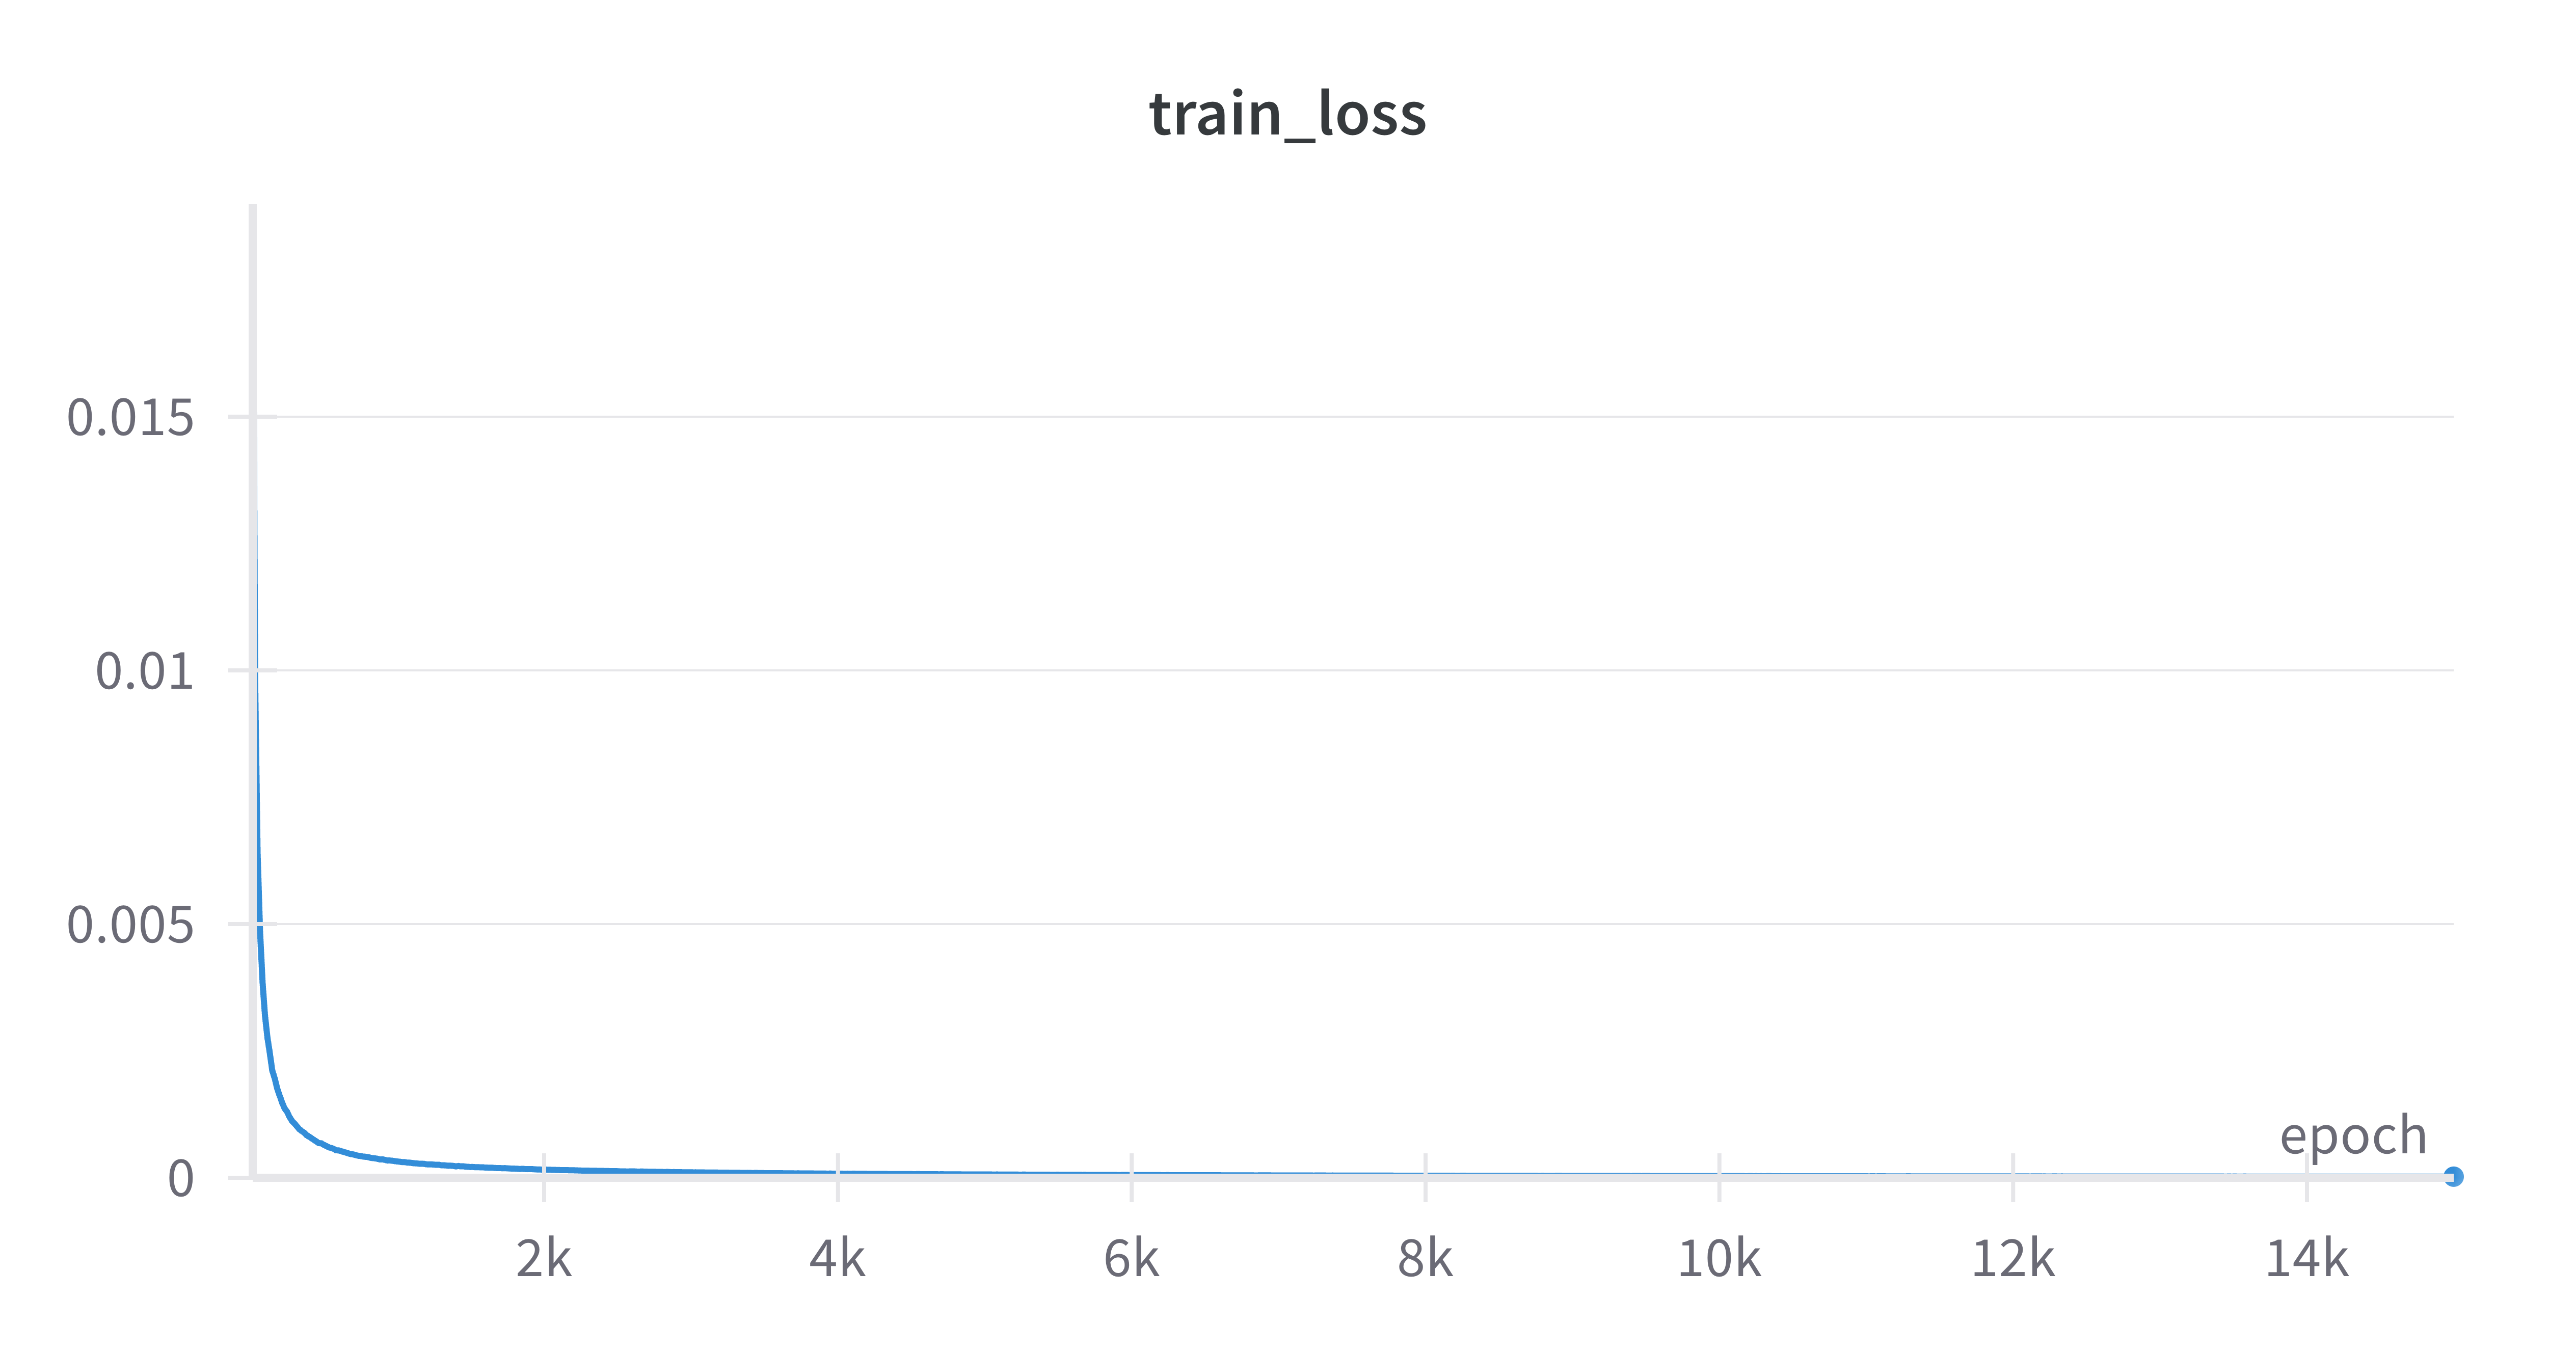
\includegraphics[width=\linewidth]{detailed_engineering/Monai Diffusion - Attempt 2/charts/train_loss.png}
\caption{}
\endminipage\hfill
\minipage{0.49\textwidth}
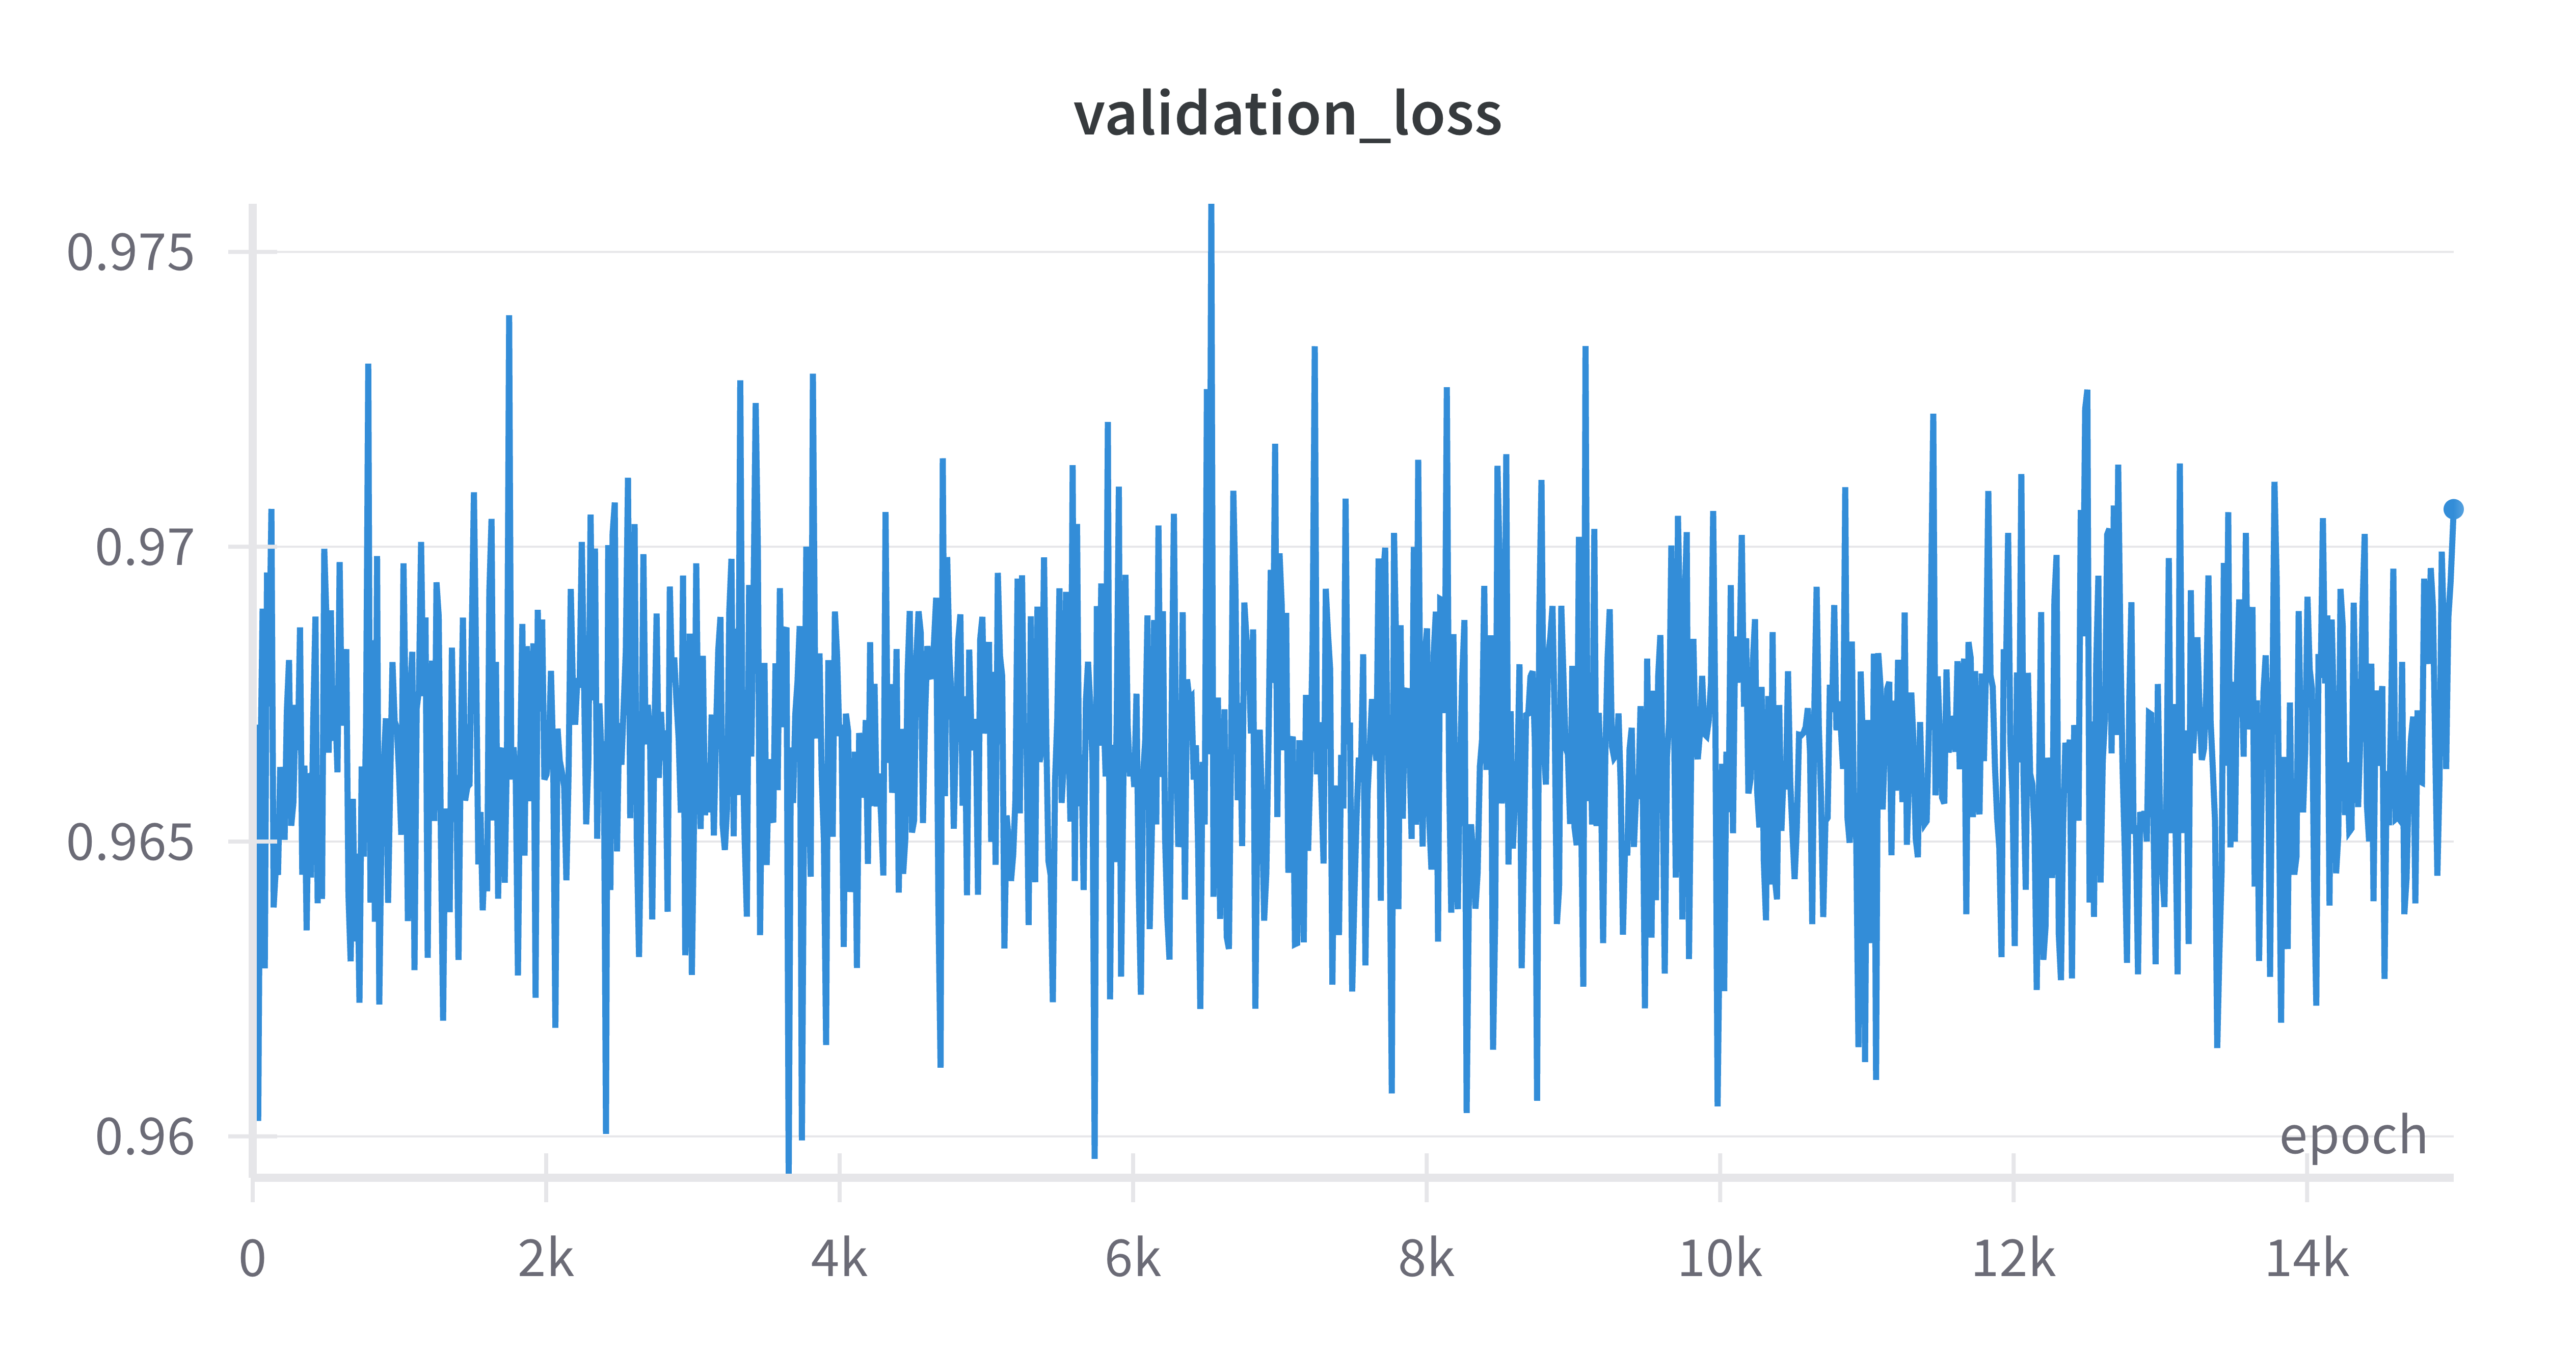
\includegraphics[width=\linewidth]{detailed_engineering/Monai Diffusion - Attempt 2/charts/validation_loss.png}
\caption{}
\label{fig:ldm_a2_val_loss}
\endminipage
\end{figure}

As is visible in the figure \ref{fig:ldm_a2_val_loss}, the validation loss did not decrease. The output of the generation was the same as in the previous attempt.




% \paragraph{Training}
% \begin{figure}[H]
% \centering
% \begin{subfigure}[h]{.45\linewidth}
%     \includegraphics[width=\linewidth]{detailed_engineering/Monai Diffusion - Attempt 1/charts/step_loss.png}
%     \caption{Caption}
%     \label{fig:enter-label}
% \end{subfigure}
% \hfill
% \begin{subfigure}[h]{.45\linewidth}
%     \includegraphics[width=\linewidth]{detailed_engineering/Monai Diffusion - Attempt 1/charts/val_loss.png}
%     \caption{Caption}
%     \label{fig:enter-label}
% \end{subfigure}
% \end{figure}

% \begin{figure}[H]
% \centering
% \begin{subfigure}[h]{.45\linewidth}
%     \includegraphics[width=\linewidth]{detailed_engineering/Monai Diffusion - Attempt 2/charts/step_loss.png}
%     \caption{Caption}
%     \label{fig:enter-label}
% \end{subfigure}
% \hfill
% \begin{subfigure}[h]{.45\linewidth}
%     \includegraphics[width=\linewidth]{detailed_engineering/Monai Diffusion - Attempt 2/charts/val_loss.png}
%     \caption{Caption}
%     \label{fig:enter-label}
% \end{subfigure}
% \end{figure}


% \hfill
% \begin{subfigure}[h]{.45\linewidth}
%     \includegraphics[width=\linewidth]{detailed_engineering/Monai Diffusion - Attempt 1/charts/}
%     \caption{Caption}
%     \label{fig:enter-label}
% \end{subfigure}
% \hfill
% \begin{subfigure}[h]{.45\linewidth}
%     \includegraphics[width=\linewidth]{detailed_engineering/Monai Diffusion - Attempt 1/charts/Section-4-Panel-3-dn8bpp6rt.png}
%     \caption{Caption}
%     \label{fig:enter-label}
% \end{subfigure}
% \hfill
% \begin{subfigure}[h]{.45\linewidth}
%     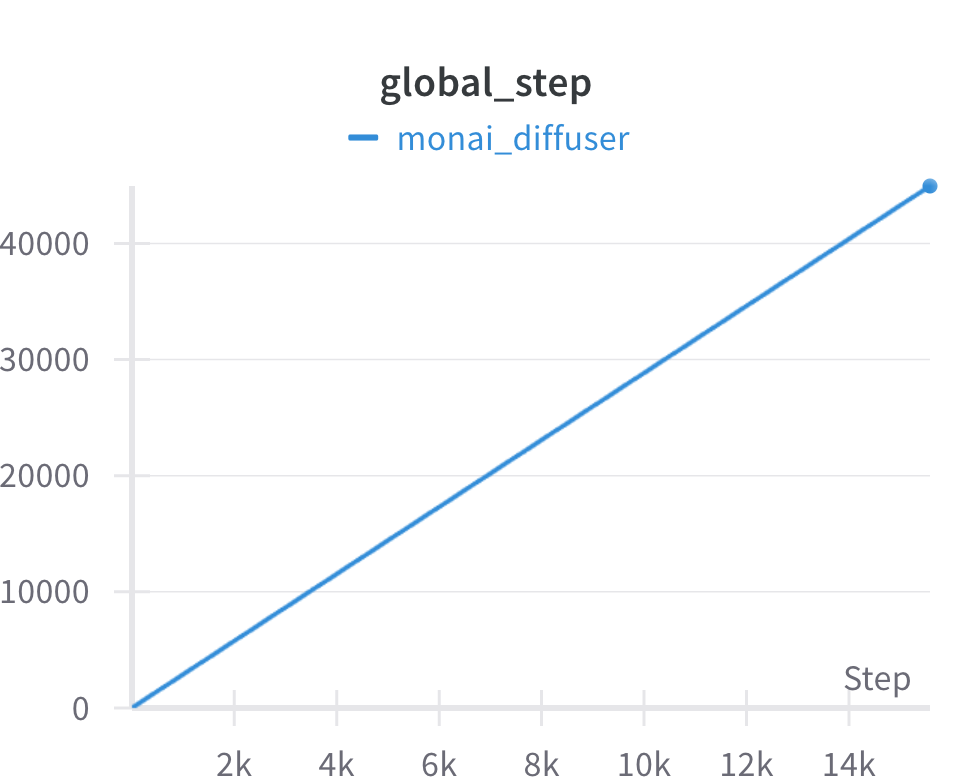
\includegraphics[width=\linewidth]{detailed_engineering/Monai Diffusion - Attempt 1/charts/Section-4-Panel-4-z2xepgyu7.png}
%     \caption{Caption}
%     \label{fig:enter-label}
% \end{subfigure}
% \begin{subfigure}[h]{.45\linewidth}
%     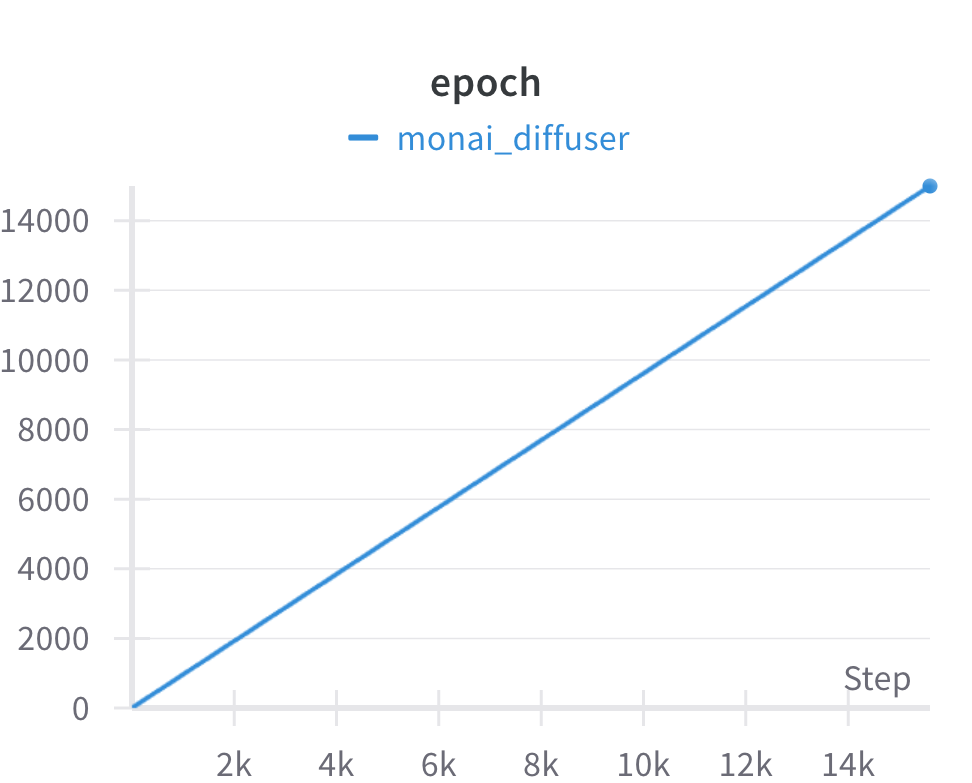
\includegraphics[width=\linewidth]{detailed_engineering/Monai Diffusion - Attempt 1/charts/Section-4-Panel-5-4t8ldmpb8.png}
%     \caption{Caption}
%     \label{fig:enter-label}
% \end{subfigure}
% \end{figure}

\paragraph{Model configuration}

\paragraph{Training}

\paragraph{Results}



